\section{Software simulator for Porous Media Problems}

\begin{frame}
	\frametitle{\secname}

	\begin{alertblock}{DUNE for Multi-\{Phase, Component, Scale, Physics, \ldots\} flow and transport in porous media (DuMu\textsuperscript{x})}
		\note{
			Título: Una introducción a la caja de herramientas DUNE en
			C++/Python para la solución de modelos matemáticos.

			Se hará una breve presentación de la caja de herramientas
			modular Dune Numerics, biblioteca modular desarrollada en la
			Universidad de Heildeberg en C++ y Python, para resolver
			ecuaciones diferenciales parciales utilizando métodos basados
			en mallas, por ejemplo diferencias finitas, elementos finitos o
			volúmenes finitos.

			Es un software de código abierto bajo la licencia GNU General
			Public Licence 2, con binarios disponibles para las
			distribuciones linux Debian, Ubuntu y openSUSE; y
			los scripts de compilación en macOS, FreeBSD, Arch Linux.

			Se mostrará la estructura general, algunos proyectos basados en
			DUNE y algunas simulaciones de modelos matemáticos que incluyen
			éste tipo de ecuaciones y sus respectivas soluciones, así como
			una implementación breve de Dune Numerics.
		}
		\begin{itemize}\small
			\item

			      DuMu\textsuperscript{x} is a multipurpose open-source simulator under the
			      \href{https://www.gnu.org/licenses/lgpl-3.0.html}{
				      GNU Lesser General Public License 3}~\lgpllicense{}.

			\item

			      DUNE is available on
			      \href{https://github.com/dune-copasi/homebrew-tap}{macOS},
			      \href{https://packages.debian.org/search?suite=sid&section=all&arch=any&searchon=sourcenames&keywords=dune-}{Debian}~\debian{},
			      \href{https://launchpad.net/~opm/+archive/ubuntu/ppa}{Ubuntu}~\ubuntu{},
			      \href{https://build.opensuse.org/search?search_text=dune-&search_for=2&name=1&attrib_type_id=}{openSUSE}~\opensuse{},
			      \href{https://aur.archlinux.org/packages/?O=0&SeB=n&K=dune-&outdated=&SB=n&SO=a&PP=50&do_Search=Ir}{Arch Linux}~\archlinux{}
			      and \href{https://www.freshports.org/search.php?stype=name&method=match&query=dune-&num=20&orderby=category&orderbyupdown=asc&search=Search&format=html&branch=head}{FreeBSD}~\freebsd{}.

			      {\fontspec[Renderer=Harfbuzz]{NotoColorEmoji.ttf}🎉}
			      DUNE Release 2.9.0 is planned for end of October 2022.

			\item

			      Porous-Medium Flow, Non-Isothermal, Free Flow, Geomechanics, Pore-Network models.
			      Multidomain, multi-component, multi-phase. Parallel, Grid Adaptivity.

				      {\fontspec[Renderer=Harfbuzz]{NotoColorEmoji.ttf}🎉}
			      Release 3.6.0 is planned for October 7, 2022.

			      \note{
				      Desarrollado con CMake, escrito en C++ con enlaces Python a través de pybind11.

			      }
		\end{itemize}
	\end{alertblock}

	\begin{minipage}{0.45\textwidth}
		\begin{figure}[ht!]
			\centering
			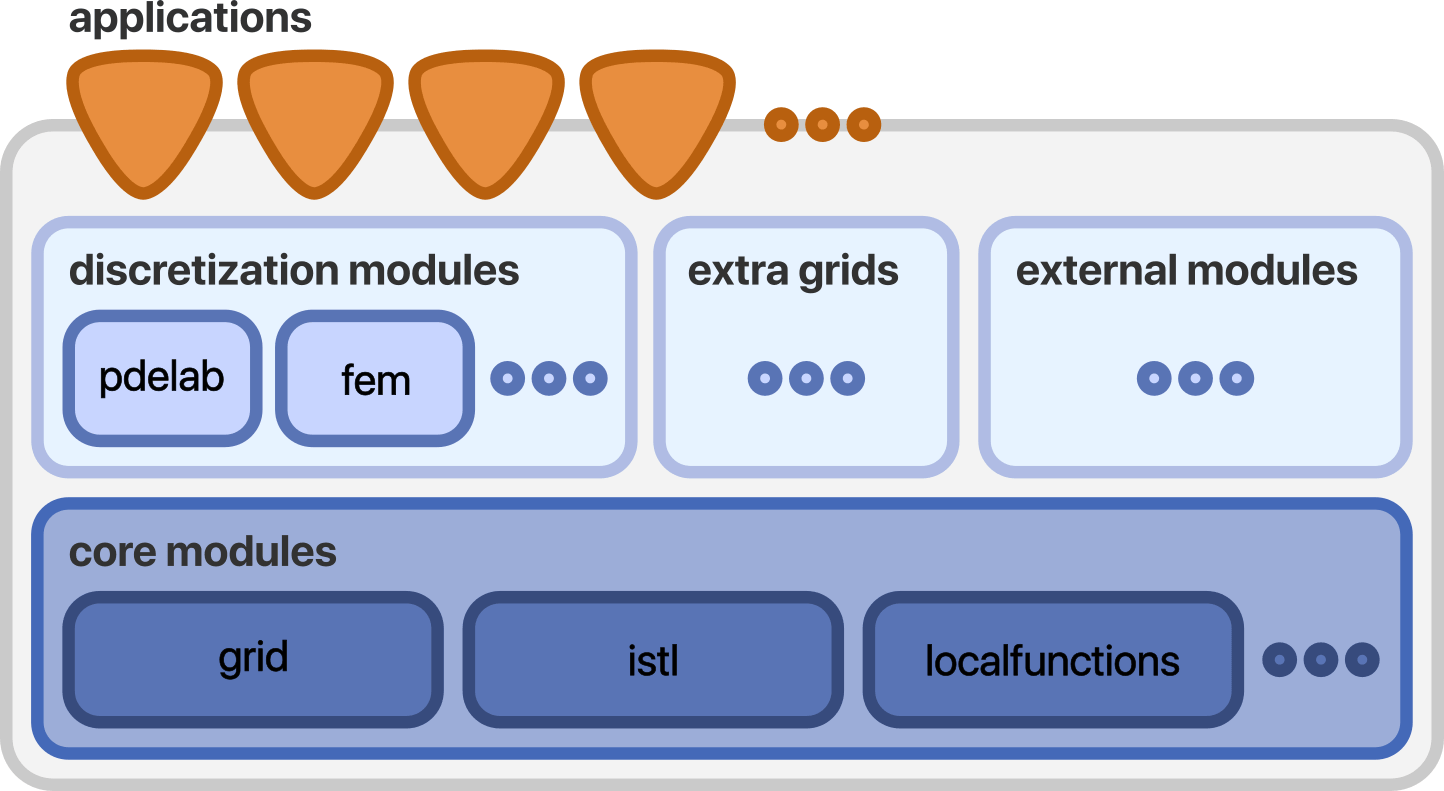
\includegraphics[height=3.2cm]{dunedesign}
			\caption{Taken from \url{https://dune-project.org}.}
		\end{figure}
	\end{minipage}\qquad\qquad
	\begin{minipage}{0.45\textwidth}
		\begin{figure}[ht!]
			\centering % https://repology.org/project/dumux/versions
			\href{https://github.com/arch4edu/arch4edu}{
\includegraphics[height=2.8cm]{arch4edu}}\quad\quad % dumux simulation picture
			\href{https://github.com/arch4edu/cactus}{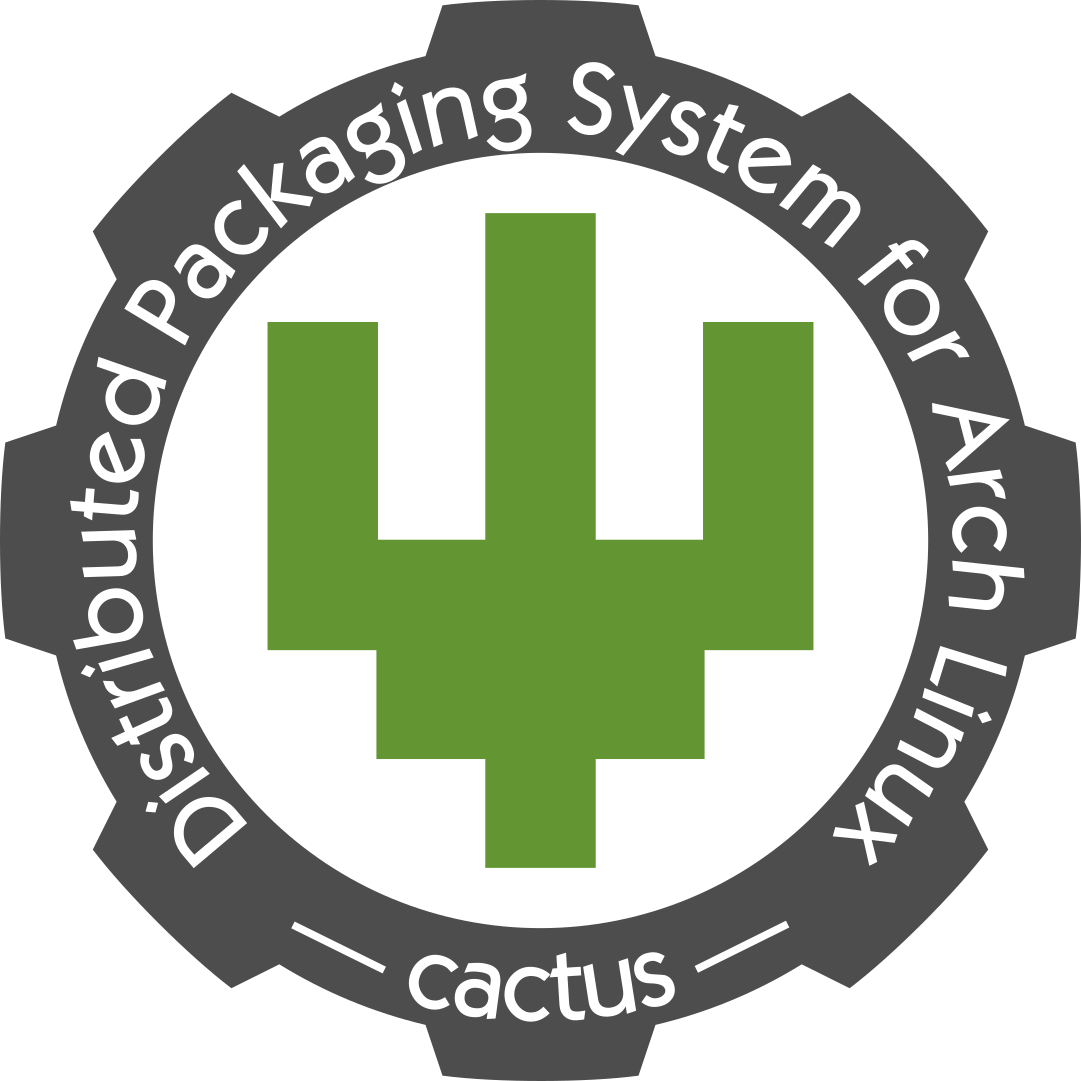
\includegraphics[height=2.8cm]{cactus.png}}
			\caption{Binaries are available in \alert{arch4edu repository} (Jingbei Li and Carlos Aznarán, 2022).}
			% The easiest way to install the binaries are from Arch Linux Repository for Education. Jingbei Li, Carlos Aznarán, et al.
		\end{figure}
	\end{minipage}

\end{frame}

% documentación https://git.iws.uni-stuttgart.de/dumux-repositories/dumux-course
% página principal
% lenguajes
% https://player.vimeo.com/video/572717824
% https://cpp-review-dune.github.io/webinar/slides.pdf
% TODO: Mirar NON-ISOTHERMAL FLUID FLOW RESERVOIR SIMULATION USING DUMUX SOFTWARE